\section{内积}
\label{sec:ipspace-inner-products}

\BookChapterRef{chap:inner-product-spaces}{卷二第4章“内积空间”}用内积定义了有限维空间中的长度、夹角和正交。内积的公理只涉及加法、数乘和取值，没有提到维数，所以可以原样放到函数和数列上。需要重新确认的是：函数上的内积具体长什么样，它给出的长度为什么是范数，以及哪些范数根本不可能来自内积。

\paragraph{内积的公理}
实空间中的内积是对称、双线性、正定的。复空间不能照搬这三条。若内积对两个变量都线性，把$x$换成$\mathrm ix$就得到
\[
 \langle\mathrm ix,\mathrm ix\rangle=\mathrm i^2\langle x,x\rangle=-\langle x,x\rangle,
\]
于是$\langle x,x\rangle$与$\langle\mathrm ix,\mathrm ix\rangle$不可能都是正数。所以复内积改用共轭对称，并且只对一个变量线性。本书与卷二一致，约定对第二个变量线性、对第一个变量共轭线性。

\begin{definition}[内积与内积空间]
\label{def:ipspace-inner-product}
设$V$是$\mathbb K$上的线性空间。映射$\langle\cdot,\cdot\rangle:V\times V\to\mathbb K$称为$V$上的\term{内积}（inner product），若对所有$f,g,h\in V$与$a,b\in\mathbb K$，
\begin{align}
 \langle h,af+bg\rangle&=a\langle h,f\rangle+b\langle h,g\rangle,
 \label{eq:ipspace-axiom-linear}\\
 \langle g,f\rangle&=\overline{\langle f,g\rangle},
 \label{eq:ipspace-axiom-conjugate}\\
 \langle f,f\rangle&\geq0,
 \label{eq:ipspace-axiom-positive}
\end{align}
且$\langle f,f\rangle=0$当且仅当$f=0$。这三条分别称为对第二个变量线性、共轭对称和正定性。配备内积的线性空间称为\term{内积空间}（inner-product space）。
\end{definition}

前两条合起来给出对第一个变量的共轭线性：
\[
 \langle af+bg,h\rangle=\bar a\langle f,h\rangle+\bar b\langle g,h\rangle.
\]
共轭对称还说明$\langle f,f\rangle$等于自己的共轭，总是实数，所以第三条的“$\geq0$”有意义。实空间中共轭不起作用，三条公理就是卷二的对称、双线性和正定性。

\paragraph{函数与数列上的内积}
先看点积怎样变成积分。把$[-1,1]$等分成$N$小段，步长$h=2/N$，取各段中点$x_1,\ldots,x_N$。函数$f$在这些点上读出一个$N$维向量$(f(x_1),\ldots,f(x_N))$，这正是“函数是无限维向量”的有限截取。两个这样的向量作点积，再乘以步长，得到
\begin{equation}
 h\sum_{i=1}^N\overline{f(x_i)}\,g(x_i)\ \xrightarrow{\ N\to\infty\ }\ \int_{-1}^1\overline{f(x)}\,g(x)\,dx .
 \label{eq:ipspace-riemann-dot}
\end{equation}
乘以$h$是必要的：不乘的话，分量越多点积越大，没有极限。

下面用$f(x)=1+x$、$g(x)=x$和$N=4$算一遍。此时$h=\tfrac12$，四个中点是$\pm\tfrac14,\pm\tfrac34$，两个函数读出的向量是
\[
 f\mapsto(0.25,\,0.75,\,1.25,\,1.75),\qquad g\mapsto(-0.75,\,-0.25,\,0.25,\,0.75).
\]
逐分量相乘再相加，得到点积
\[
 -0.1875-0.1875+0.3125+1.3125=1.25 .
\]
乘以步长$h=\tfrac12$，得到$0.625$。

精确的积分是
\[
 \int_{-1}^1(1+x)x\,dx=\int_{-1}^1x\,dx+\int_{-1}^1x^2\,dx=\frac23 .
\]
取$N=8$和$N=16$，同样的计算分别给出$0.65625$和$0.6640625$，逐渐接近$\tfrac23$。图~\ref{fig:ipspace-sampled-dot-product}画出了$N=4$时的情形：左边是两组读出的分量，右边每个矩形的高是一对分量的乘积，矩形的带符号总面积就是式~\eqref{eq:ipspace-riemann-dot}左边的和。

\begin{BookInlineFigure}
  \centering
  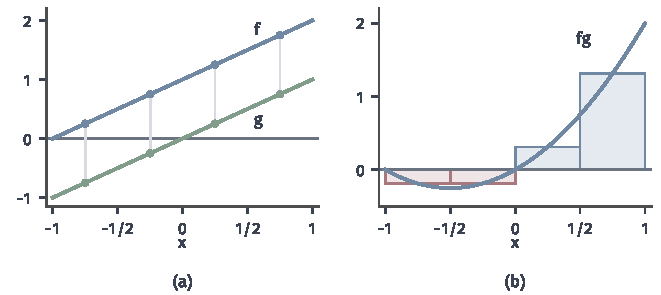
\includegraphics[width=112mm]{figures/04-spaces-measures-and-geometry/03-function-spaces/matplotlib/ipspace-sampled-dot-product/figure.pdf}
  \caption{从点积到积分内积，$f=1+x$（蓝），$g=x$（绿），$N=4$。(a)四个中点上读出的分量。(b)矩形的高是分量的乘积$f(x_i)g(x_i)$（负值用红色），宽是步长$\tfrac12$，带符号总面积$0.625$；曲线是$fg$，其下带符号面积是内积$\tfrac23$。}
  \label{fig:ipspace-sampled-dot-product}
\end{BookInlineFigure}

这个极限提示了$C[a,b]$上的内积：
\begin{equation}
 \langle f,g\rangle=\int_a^b\overline{f(x)}\,g(x)\,dx .
 \label{eq:ipspace-continuous-inner-product}
\end{equation}
实函数时共轭可以省去。对第二个变量的线性和共轭对称来自积分的线性。

正定性要用到连续性。被积函数非负，所以
\[
 \langle f,f\rangle=\int_a^b\lvert f\rvert^2\,dx\geq0 .
\]
若$f(x_0)\neq0$，由连续性存在长度为正的小区间，在其上$\lvert f\rvert\geq\tfrac12\lvert f(x_0)\rvert$，积分至少是区间长度乘$\tfrac14\lvert f(x_0)\rvert^2$，严格为正。

这里类比也开始失效。有限维向量的每个分量都带着正的权重，改动一个分量，长度就变了。积分内积中单个点的权重趋于零，改动一个点的值不影响积分。在连续函数上，连续性阻止了这种改动；一旦离开连续函数，正定性就要靠第~\ref{sec:ipspace-l2-space}节的等价类来恢复。

数列是更直接的无限维向量，下标集是$\mathbb N_+$，内积就是点积把求和号延伸到无穷：$\sum_k\overline{x_k}y_k$。麻烦在于和可能发散，比如$(1,1,1,\ldots)$与自己的点积。在有限支撑数列空间$c_{00}$上不会有这个问题，求和只有有限项非零，
\begin{equation}
 \langle x,y\rangle=\sum_k\overline{x_k}\,y_k
 \label{eq:ipspace-c00-inner-product}
\end{equation}
是内积。容纳无穷多项非零的数列要等到第~\ref{sec:ipspace-l2-space}节的$\ell^2$。

共轭在函数上同样不能省略。在$[-\pi,\pi]$上取$f(x)=e^{\mathrm ix}$，这是一个处处模长为$1$的非零函数。若不取共轭，
\[
 \int_{-\pi}^{\pi}f(x)\,f(x)\,dx=\int_{-\pi}^{\pi}e^{2\mathrm ix}\,dx=0,
\]
一个非零函数与自己的“内积”竟然为零。取共轭后被积函数变成$\lvert e^{\mathrm ix}\rvert^2=1$，于是$\langle f,f\rangle=2\pi$。

若$\langle f,g\rangle=0$，称$f$与$g$\term{正交}（orthogonal）。这里的“垂直”指乘积的整体积分为零，与两条曲线在平面上的交角无关。在$[-1,1]$上，$1$与$x$正交，$1$与$x^2$不正交，因为
\[
 \int_{-1}^1x\,dx=0,\qquad \int_{-1}^1x^2\,dx=\frac23 .
\]
正交还依赖积分区间：换到$[0,1]$上，$\int_0^1x\,dx=\tfrac12$，$1$与$x$就不再正交了。

\paragraph{Cauchy--Schwarz不等式与诱导范数}
内积给出长度$\lVert f\rVert=\sqrt{\langle f,f\rangle}$。要说明它是范数，关键在三角不等式，而三角不等式依赖下面这个不等式。

它的几何图景是：$\mathbb R^3$中把$f$投影到$g$所在的直线上，垂线段的长度不小于零，由此得到$\cos\theta$的绝对值不超过$1$。证明就是把这幅图写成计算，用到的只有内积公理，与维数无关。

\begin{theorem}[Cauchy--Schwarz不等式]
\label{thm:ipspace-cauchy-schwarz}
在内积空间中，对所有$f,g$，
\begin{equation}
 \lvert\langle f,g\rangle\rvert\leq\lVert f\rVert\,\lVert g\rVert ,
 \label{eq:ipspace-cauchy-schwarz}
\end{equation}
等号当且仅当$f,g$线性相关。
\end{theorem}

\begin{proof}
若$g=0$，两边都为零，$f,g$线性相关。下面设$g\neq0$。

取$f$在$g$方向上的影子$\alpha g$，其中$\alpha=\langle g,f\rangle/\lVert g\rVert^2$。这个系数使余量$f-\alpha g$与$g$正交：
\[
 \langle g,f-\alpha g\rangle=\langle g,f\rangle-\alpha\lVert g\rVert^2=0 .
\]

展开余量长度的平方时，先把第二个变量拆开。含$g$的那一项因为上面的正交关系而消失，于是
\[
 \lVert f-\alpha g\rVert^2=\langle f-\alpha g,f\rangle=\lVert f\rVert^2-\bar\alpha\langle g,f\rangle .
\]

代入$\bar\alpha=\langle f,g\rangle/\lVert g\rVert^2$。$\langle f,g\rangle$与$\langle g,f\rangle$互为共轭，乘积是模的平方，于是
\[
 0\leq\lVert f-\alpha g\rVert^2=\lVert f\rVert^2-\frac{\lvert\langle f,g\rangle\rvert^2}{\lVert g\rVert^2}.
\]
移项开方即得不等式。等号成立当且仅当$\lVert f-\alpha g\rVert=0$，即$f=\alpha g$；反过来，若$f=cg$，直接代入可知$\alpha=c$，等号成立。
\end{proof}

用$[0,1]$上的$f=1$、$g=x$核对一下。三个内积是
\[
 \langle f,g\rangle=\frac12,\qquad \lVert f\rVert^2=1,\qquad \lVert g\rVert^2=\frac13 .
\]
不等式成为$\tfrac12\leq\tfrac1{\sqrt3}\approx0.577$。影子的系数是$\alpha=\tfrac12\big/\tfrac13=\tfrac32$，余量$1-\tfrac32x$的长度平方是
\[
 \int_0^1\Bigl(1-\frac32x\Bigr)^2dx=1-\frac32+\frac34=\frac14,
\]
与证明中的公式给出的$1-\tfrac34$相同。

在实空间中，式~\eqref{eq:ipspace-cauchy-schwarz}保证下面的比值落在$[-1,1]$内，可以用它定义函数之间的夹角：
\[
 \cos\theta=\frac{\langle f,g\rangle}{\lVert f\rVert\,\lVert g\rVert}.
\]
上面的$1$与$x$在$[0,1]$上的夹角满足$\cos\theta=\tfrac{\sqrt3}2$，即$\theta=30^\circ$；在$[-1,1]$上内积为零，夹角是$90^\circ$。

三角不等式现在可以推出。把$\lVert f+g\rVert^2$按内积展开，再用Cauchy--Schwarz不等式放大交叉项：
\[
 \begin{aligned}
 \lVert f+g\rVert^2&=\lVert f\rVert^2+2\operatorname{Re}\langle f,g\rangle+\lVert g\rVert^2\\
 &\leq\lVert f\rVert^2+2\lVert f\rVert\,\lVert g\rVert+\lVert g\rVert^2\\
 &=(\lVert f\rVert+\lVert g\rVert)^2 .
 \end{aligned}
\]
齐次性$\lVert cf\rVert=\lvert c\rvert\,\lVert f\rVert$与正定性直接来自内积公理。所以每个内积空间都是赋范空间，这个范数称为内积的\term{诱导范数}（induced norm）。在$C[a,b]$上，它就是平方积分大小$\bigl(\int_a^b\lvert f\rvert^2\,dx\bigr)^{1/2}$。

Cauchy--Schwarz不等式还说明内积对两个变量连续。把差拆成只改一个变量的两项：
\[
 \langle f_n,g_n\rangle-\langle f,g\rangle=\langle f_n-f,g_n\rangle+\langle f,g_n-g\rangle .
\]
对每一项用不等式~\eqref{eq:ipspace-cauchy-schwarz}，得到
\begin{equation}
 \lvert\langle f_n,g_n\rangle-\langle f,g\rangle\rvert\leq\lVert f_n-f\rVert\,\lVert g_n\rVert+\lVert f\rVert\,\lVert g_n-g\rVert .
 \label{eq:ipspace-inner-continuity}
\end{equation}
若$f_n\to f$、$g_n\to g$，$\lVert g_n\rVert$有界，右边趋于零，所以$\langle f_n,g_n\rangle\to\langle f,g\rangle$。后面凡是在极限中保持正交关系，用的都是这一点。

\paragraph{平行四边形恒等式}
内积范数比一般范数多一条性质。在平面上，平行四边形两条对角线的平方和等于四条边的平方和。这条几何事实在内积空间中照样成立：
\begin{equation}
 \lVert f+g\rVert^2+\lVert f-g\rVert^2=2\lVert f\rVert^2+2\lVert g\rVert^2 ,
 \label{eq:ipspace-parallelogram}
\end{equation}
称为\term{平行四边形恒等式}（parallelogram identity）。验证时把左边两项按内积展开，交叉项$2\operatorname{Re}\langle f,g\rangle$与$-2\operatorname{Re}\langle f,g\rangle$相互抵消，剩下的正是右边。

一般的范数未必满足它，因此未必来自内积。在$C[0,1]$上取一致范数，令$f=1$、$g=x$。这时$f+g=1+x$的最大值是$2$，$f-g=1-x$的最大值是$1$，于是
\[
 \lVert f+g\rVert_\infty^2+\lVert f-g\rVert_\infty^2=4+1=5 .
\]
而$\lVert f\rVert_\infty=\lVert g\rVert_\infty=1$，右边是
\[
 2\lVert f\rVert_\infty^2+2\lVert g\rVert_\infty^2=4 .
\]

$L^1$范数同样不满足。在$L^1[0,1]$中取两半区间的指示函数$f=\mathbf 1_{[0,1/2]}$、$g=\mathbf 1_{(1/2,1]}$，有
\[
 \lVert f+g\rVert_1=\lVert f-g\rVert_1=1,\qquad \lVert f\rVert_1=\lVert g\rVert_1=\frac12 .
\]
左边等于$2$，右边等于$1$。两个范数都违反式~\eqref{eq:ipspace-parallelogram}，所以没有任何内积能诱导它们。

反过来，满足平行四边形恒等式的范数一定来自内积。实情形下这个内积只能是
\begin{equation}
 \langle f,g\rangle=\frac14\bigl(\lVert f+g\rVert^2-\lVert f-g\rVert^2\bigr) ,
 \label{eq:ipspace-polarization}
\end{equation}
因为按内积展开右边，正好只剩$\langle f,g\rangle$。证明这个式子确实定义了内积，需要由恒等式逐步推出可加性，再把齐次性从有理数推广到实数，篇幅较长，读者可在泛函分析教材中查阅Jordan--von Neumann定理。本章只用正方向：内积范数满足式~\eqref{eq:ipspace-parallelogram}，它将是第~\ref{sec:ipspace-orthogonal-projection}节证明最近点存在的关键。
